Personalizability consists of two aspects: constraints and preferences.
From the viewpoint of the planner,
constraints, also referred to as hard constraints, are statements that the planner
has to satisfy during the planning process; whereas preferences, also called
soft constraints, are specifications that the planner will need to optimize.
We formulated constraints using linear temporal logic (LTL) and preferences as
a preferential cost function (PCF), and implemented our planner leveraging the
widely-used graph search algorithm the A*.

\subsection{Constraints}
%\begin{itemize}
%	\setlength\itemsep{1pt}
%	\item Describe syntax and semantics of LTL in the setting of trip planning.
%	\begin{itemize}
%		\setlength\itemsep{0pt}
%		\item Specifically, we need to point out the ``after" temporal connective,
%					and we need to describe the semantics: what is a plan, why we can
%					eliminate actions and put them as state attributes instead, etc.
%	\end{itemize}
%\end{itemize}
As constraints in the setting of trip planning are often declarative and
temporal, our choice of LTL is straightforward.
We now give a brief review of linear temporal logic (LTL).
Let $f$ be a propositional formula over a finite set $L$ of Boolean variables.  
LTL formulas are defined recursively as follows.
\begin{equation}
	\varphi = f | \varphi_1 \land \varphi_2 | \varphi_1 \lor \varphi_2 | \neg \varphi | 
		\bigcirc \varphi |	\Box \varphi | \Diamond \varphi | \varphi_1 \cA \varphi_2
\end{equation}
Note that we have $\varphi_1 \cA \varphi_2$, and it means that
``$\varphi_2$ holds right after $\varphi_1$ holds."

A natural constraint in trip planning could be ``In this trip I will not drive a car 
after biking or taking the public transit."
In LTL, such constraint can be translated into an LTL formula
\begin{equation}
\label{eqt:ex}
	\psi = ((M=b) \lor (M=p)) \,\cA\, (\Box (\neg (M=c))).
\end{equation}

As the actions in trip planning is limited to taking different transportation modes,
in our definition of the semantics of LTL
these actions are subsumed into the interpretations of $L$, or \tit{states}.
The semantics of LTL is defined with regard to trajectories of states. 
Let $\sigma$ be a trajectory of states $S_0,a_1,S_1,\ldots,a_n,S_n$, and
$\sigma[i]$ a suffix $S_i, a_{i+1}, S_{i+1}, \ldots,a_n,S_n$.  We have
\begin{align*}
	\sigma \models f \;\; &\IFF \;\; S_0 \models f,\\
	\sigma \models \varphi_1 \land \varphi_2 \;\; &\IFF \;\; \sigma \models \varphi_1 \; and \; \sigma \models \varphi_2,\\
	\sigma \models \varphi_1 \lor \varphi_2 \;\; &\IFF \;\; \sigma \models \varphi_1 \; or \; \sigma \models \varphi_2,\\
	\sigma \models \neg \varphi \;\; &\IFF \;\; \sigma \not \models \varphi,\\
	\sigma \models \bigcirc \varphi \;\; &\IFF \;\; \sigma[1] \models \varphi,\\
	\sigma \models \Box \varphi \;\; &\IFF \;\; \forall 0 \leq i \leq n (\sigma[i] \models \varphi),\\
	\sigma \models \Diamond \varphi \;\; &\IFF \;\; \exists 0 \leq i \leq n (\sigma[i] \models \varphi),\\
	\sigma \models \varphi_1 \cA \varphi_2 \;\; &\IFF \;\; \forall 0 \leq i < n (\IF \; \sigma[i] \models \varphi_1, \sigma[i+1] \models \varphi_2).
\end{align*}

For example, we are given an LTL constraint $\psi$ and three trajectories ($\sigma_1$, $\sigma_2$ and $\sigma_3$)
as shown in \figref{trjs}.
Clearly, we have $\sigma_1 \models \psi$ because, after public transit in $S_2$ and $S_3$, 
traveling by car has never been taken place.
Moreover, we have $\sigma_2 \not \models \psi$ because we have $M=c$ hold in $S_6$ and $S_7$
after having $M=p$ hold in $S_2$ and $S_5$.
Finally, we know $\sigma_3 \models \psi$, as the mode is always neither biking nor public transit.

\begin{figure}[!ht]
  \centering
    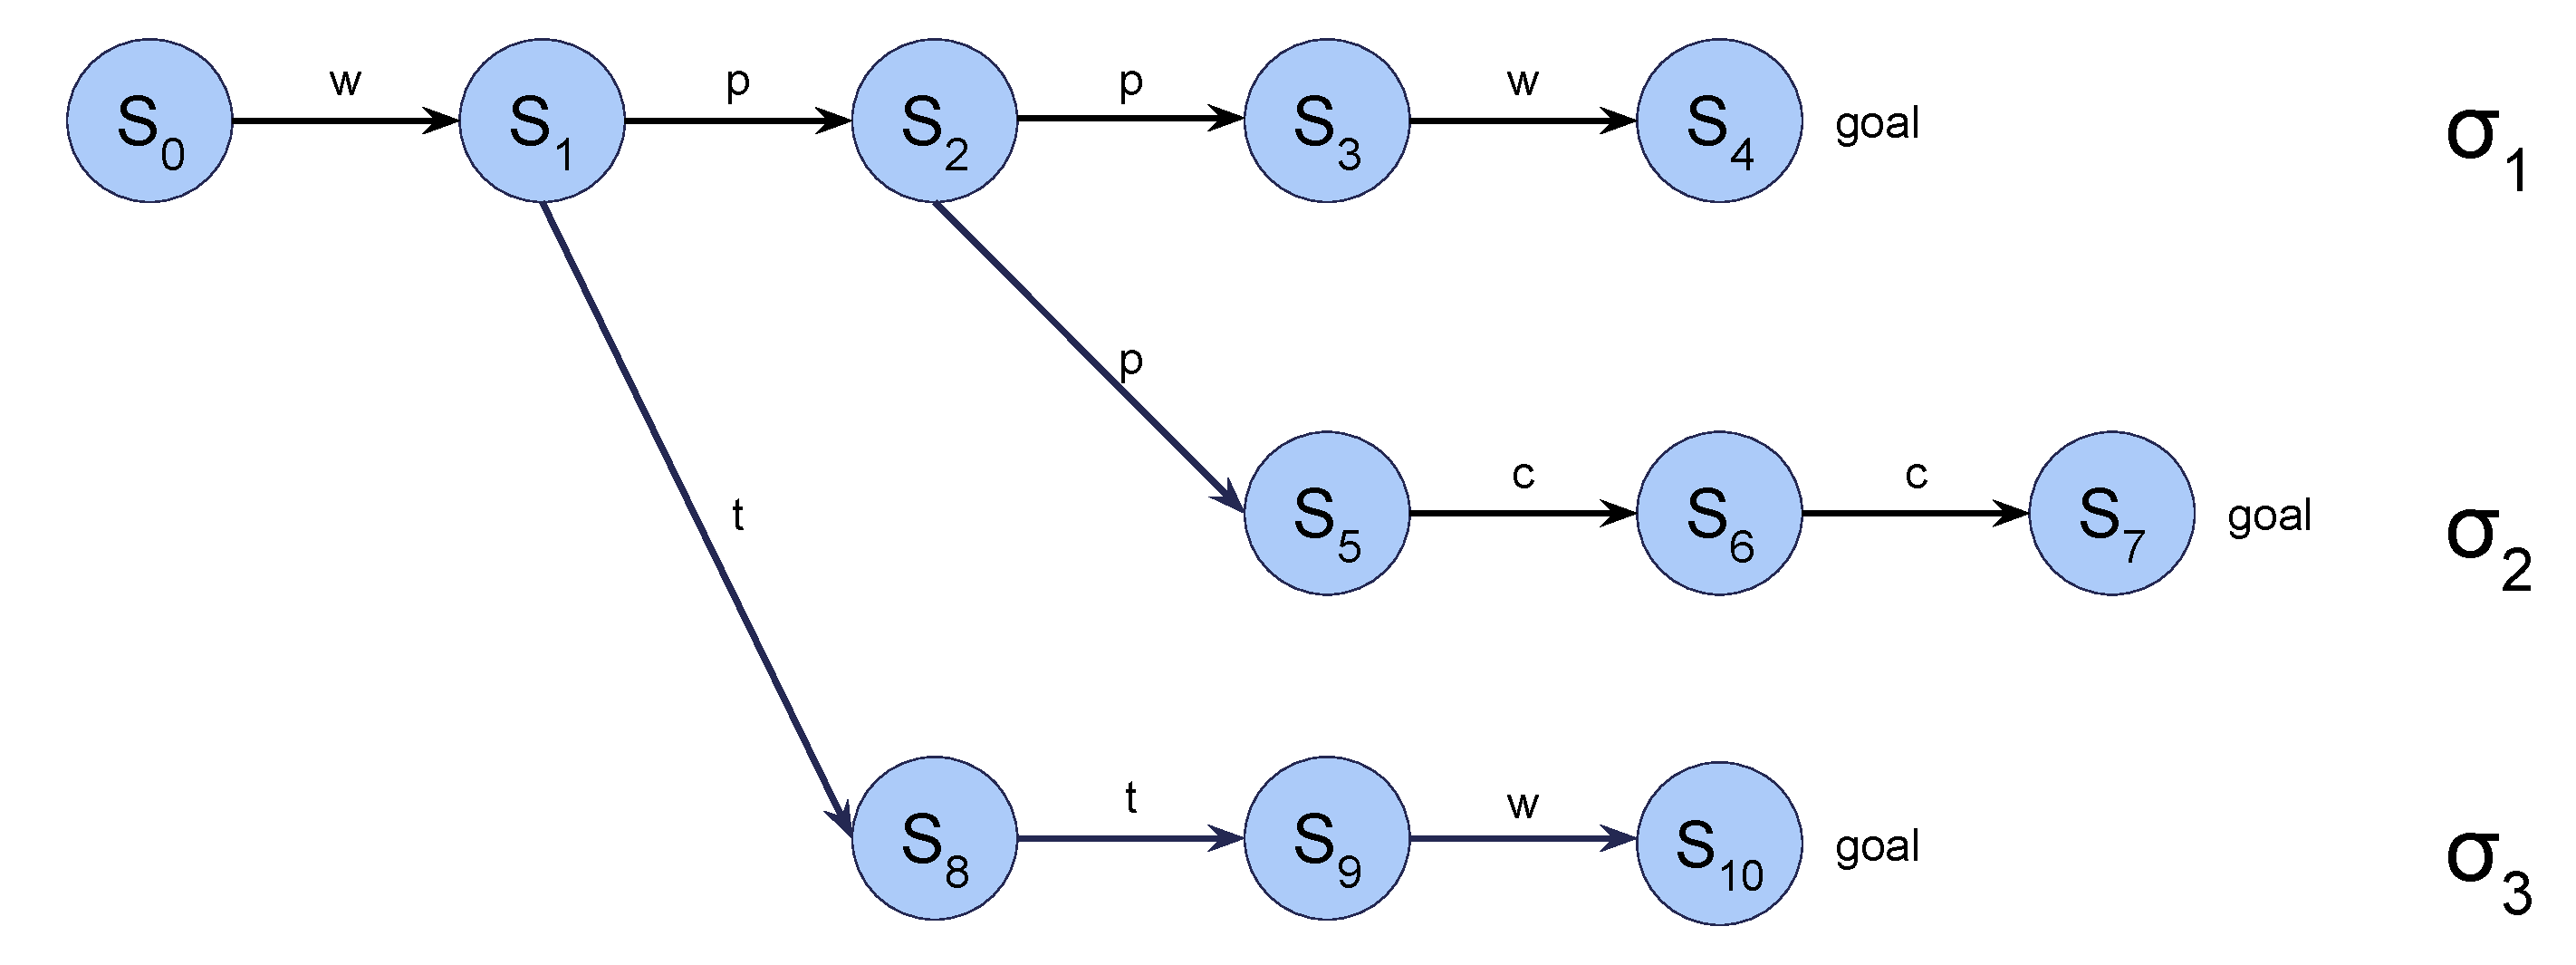
\includegraphics[width=0.4\textwidth]{figs/trajectories.pdf}
  \caption{State transition diagram\label{fig:trjs}}
\end{figure}


\subsection{Preferences}
%\begin{itemize}
%	\setlength\itemsep{1pt}
%	\item Describe our preferential cost function (PCF).
%	\begin{itemize}
%		\setlength\itemsep{0pt}
%		\item Describe why and how we break down time and money.
%		\item Describe why and how we design coefficients to these time and money pieces.
%		\item Describe why and how we design the two ratios: dollars per hour and dollars per aux.
%	\end{itemize}
%\end{itemize}

A state is described as a set of \tit{state variables}.
The state variables of a state $S$ include the transportation mode $M$ that led to $S$,
time $T$ spent so far per mode (e.g., $T_\bike$ for biking and $T_\public$ for
public transit), fare $D$ spent so far per mode (e.g., $D_\gas$ for driving and
$D_\taxi$ for taking a cab), and variables related to the auxiliary data once uploaded.
These extra data related variables are metrics such as the sum ($A_\SUM$),
the maximum ($A_\MAX)$, the minimum ($A_\MIN$), and the average ($A_\AVG$) data along the path.

We focused on weighted functions over state variables and
designed the cost function, called preferential cost function (PCF), that guides the
graph-based search engine in our trip planner as follows.
\begin{equation}
	\begin{aligned}
		\PCF(S) =& \beta_1 * (\alpha_\walk \cdot T_\walk + \alpha_\bike \cdot T_\bike + \ldots) \\
								&+ (D_\gas + D_\public + \ldots) \\
								&+ \beta_2 * (A_\SUM + \ldots),
	\end{aligned}
	\label{eqt:pcf}
\end{equation}
where $\alpha_i$ are real numbers representing the relations among different time pieces,
and $\beta_1$ ($\beta_2$) is the ratio that essentially describes how much in dollars a user would pay to
save an hour (an auxiliary data, respectively).

\subsubsection{Preference Elicitation}
To gather these coefficients ($\alpha_i$'s and $\beta_i$'s) in our $\PCF$, we designed interface to
elicit these numbers from the user.
It asks the user questions and collect answers from the user to derive the coefficients.
These questions are as follows.
\begin{enumerate}
	\item One hr of walking $=$ \underline{\hspace{1cm}} hrs of driving?
	\item One hr of biking $=$ \underline{\hspace{1cm}} hrs of driving?
	\item One hr of public transit $=$ \underline{\hspace{1cm}} hrs of driving?
	\item One hr of taxi $=$ \underline{\hspace{1cm}} hrs of driving?
	\item How much in dollars would you pay to save an hour in traveling?
	\item How much in dollars would you pay to avoid an auxiliary event (e.g., crime) in traveling?
\end{enumerate}
For instance, Alice, an agent, answers 3, 2, 0.25 and 0.5 to the first four questions in the list above.
Intuitively, the numbers indicate that she prefers public transit the most, followed by
taxi, driving, biking and walking, in order.
We show how we can now derive $\alpha_i$'s in \eqtref{pcf}.
We start with setting $\alpha_\car=1$.
Now, since one hour of walking is equivalent to 3 hours of walking,
we have $\alpha_\walk \times 1 = \alpha_\car \times 3$;
hence, we derive $\alpha_\walk = 3$.
Similarly, we have $\alpha_\bike = 2$, $\alpha_\public = 0.25$,
and $\alpha_\taxi = 0.5$.
Computing $\beta_1$ and $\beta_1$ is straightforward.
Indeed, function $\PCF$ with the input of time, fare and
auxiliary metric pieces boils down to monetary cost,
and the planner computes the best path by optimize
based on this overall monetary cost in the searching
process.

\subsection{Reasoning with Constraints and Preferences}
%\begin{itemize}
%	\setlength\itemsep{1pt}
%	\item Describe why and how we integrate constraints and preferences into A*.
%\end{itemize}

\begin{figure}[!ht]
  \centering
    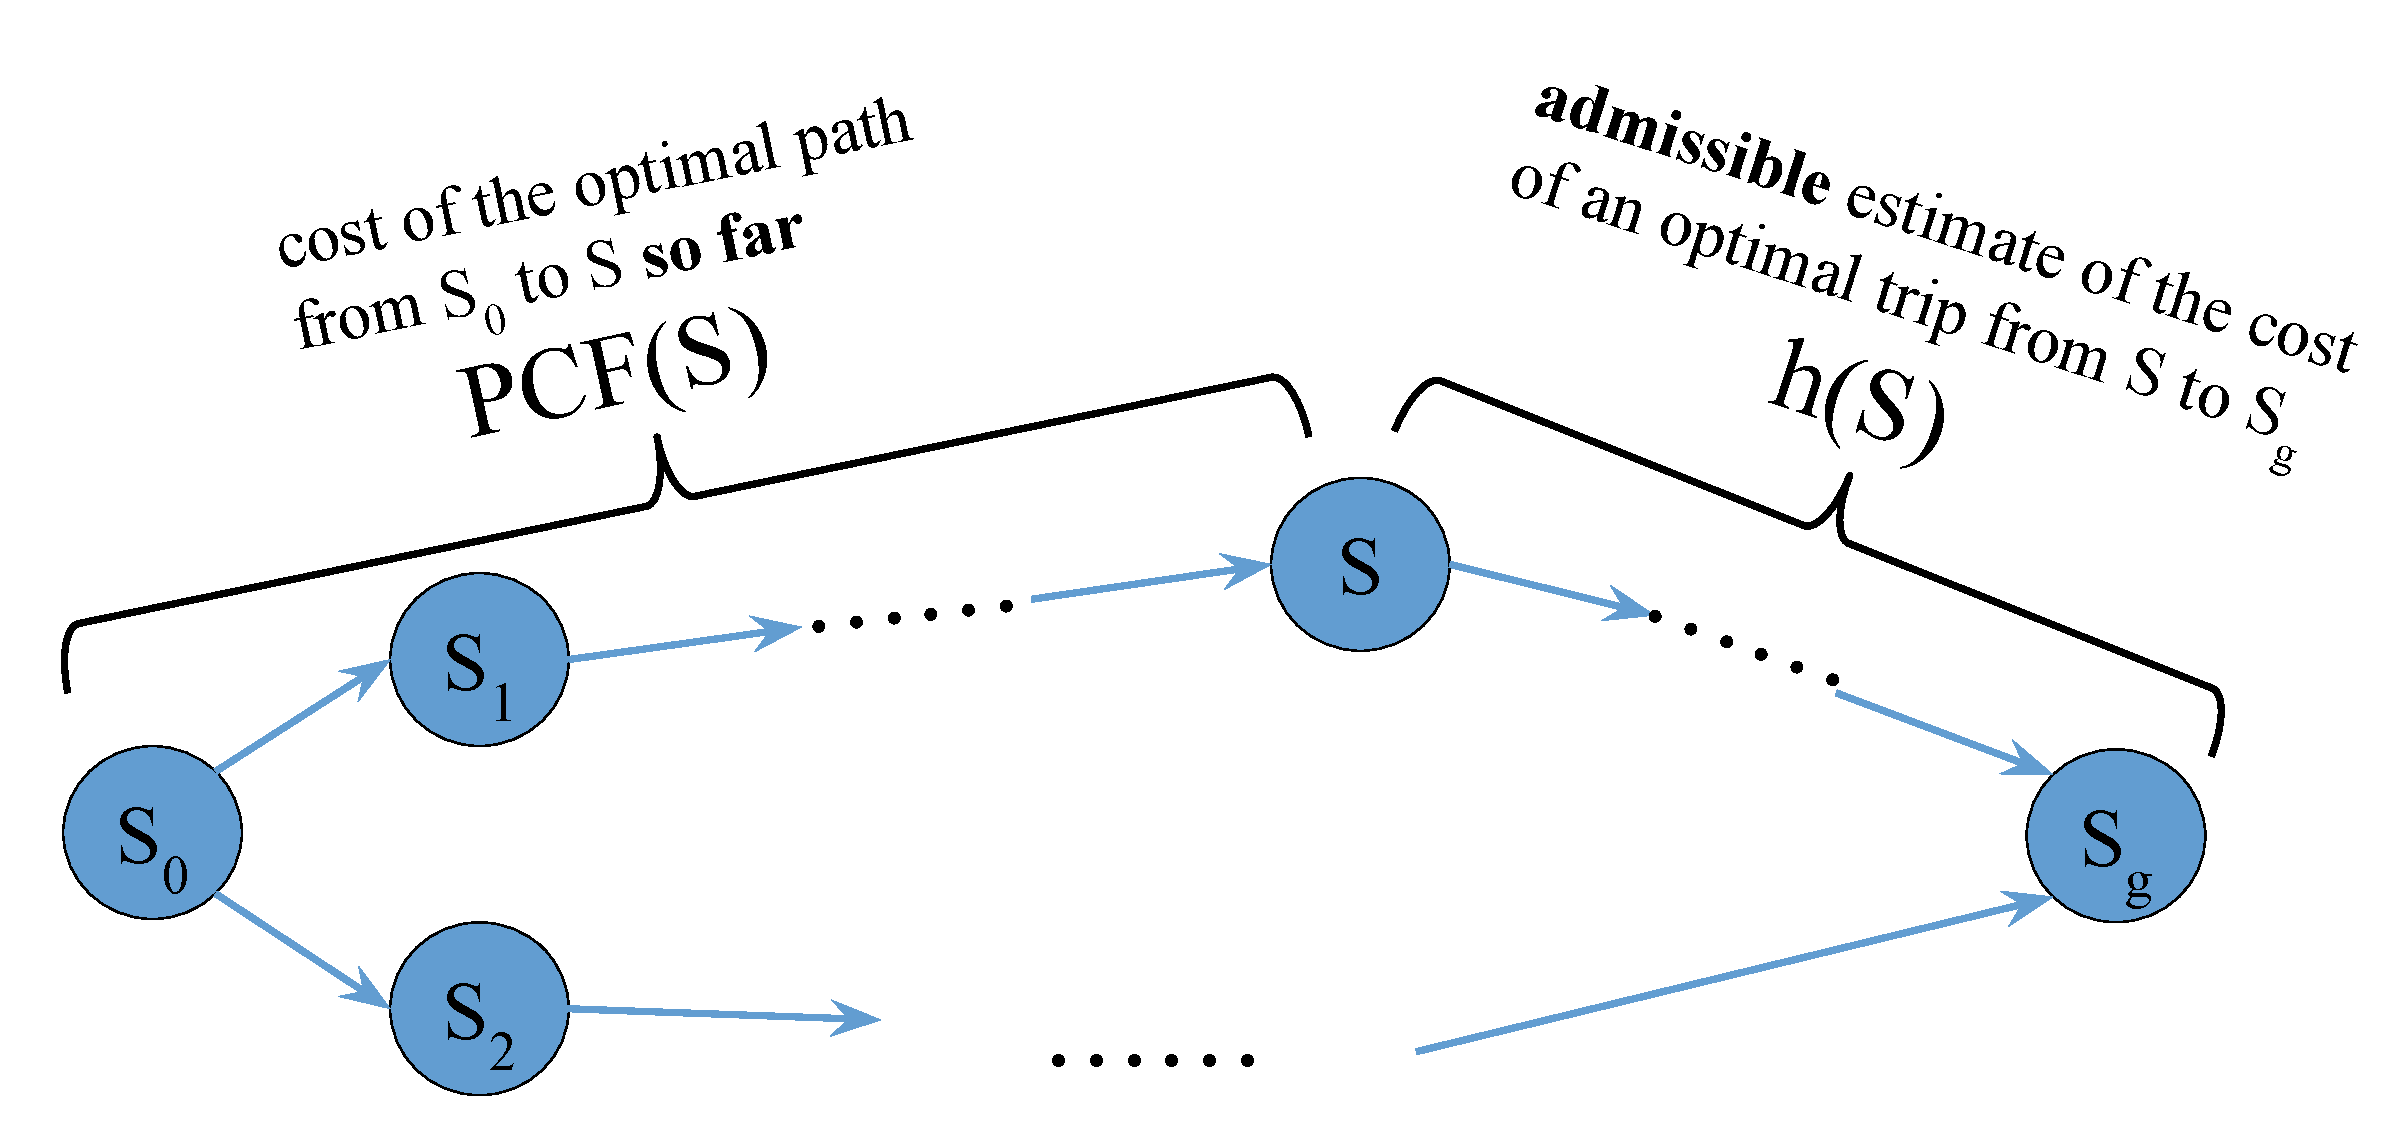
\includegraphics[width=0.4\textwidth]{figs/Astar.pdf}
  \caption{Adjusted A*\label{fig:astar}}
\end{figure}

We leveraged the widely-used A* search algorithm on top of our high-performance graph search
engine (cf. \figref{astar}).  The A* algorithm incorporates the following cost function.
\begin{equation}
	f(S) = g(S) + h(S),
\end{equation}
where $g(S)$ is the cost of an optimal trip from the initial state to $S$, and
$h(S)$ is an admissible estimate of the cost of an optimal trip from $S$ to goal.

To prune the search space, we check satisfiability of the temporal constraints in LTL
at expansion of the search tree.
To guide the search engine, we set $g(S)=\PCF(S)$ and $h(S)$ the minimum estimate among
all available modes in $S$.
